\lab{Complex Integration}{Integration in the Complex Plane}

\objective{Understand some simple uses of residues and singularities in the complex plane.}

In Lab \ref{Lab:complex_intro} we demonstrated the fact that integrals of holomorphic functions are independent of path.
Here we will consider the effect that singularities have on this property.

\section*{Laurent Series and Singular Points}

We will now introduce another form of series representation of functions.
A Laurent series of a function is a series of the form
\[\sum_{n= -\infty}^{\infty} a_n (z-z_0)^n\]
It can be proven that
\[a_n = \frac{1}{2\pi i} \int_C \frac{f(z)}{(z-z_0)^{n+1}} dz\]
Where $C$ is a contour which passes counterclockwise around the singularity exactly once.
When $f$ does not have a singularity at $z_0$ this representation degenerates to a normal Taylor Series (with the derivatives evaluated by the formula for the $n$th derivative of an analytic function).
These sorts of series are considered in greater detail in the text.
The built in function \li{sympy.series} can evaluate the series expansion of a function at a singularity, for example
\begin{lstlisting}
import sympy as sy
z = sy.Symbol('z')
(1/sy.sin(z)).series(z,0,8)
\end{lstlisting}

The Laurent series representation provides a simple way to classify singularities in the complex plane.
Isolated singular points can be classified as removable singular points, poles, or essential singular points.
These definitions will also be discussed in greater detail in the text.
Here we will show another method for visualizing complex functions.
In Lab \ref{Lab:complex_intro} we presented color plots as a useful method for visualizing functions in the complex plane. 
Here we will also show how to use surface plots to visualize the modulus of complex functions.

Now you have to take care when a surface plot is about a singularity.  We must account for the fact that the function is not going to be defined at all of the points we use in our graph.
We will also have to limit the $z$ axis on the plot to avoid creating a plot that is dominated exclusively by the extremely large and extremely small values of the function.
Plotting libraries like Mayavi and Matplotlib do allow thresholding of 3D plots via the use of floating point values of \li{nan}, but doing this may result in graphs having jagged edges where they have been cut.
We can avoid the jagged edges by artificially adding a small lip of constant values to the plot as well.
This can be done with Matplotlib as follows:
\begin{lstlisting}
import numpy as np
from mayavi import mlab

mn, mx = -1, 1
res = 400
# Set the threshold at which to cut the 'z' values
threshold = 2.
# space in 'z' values to use to create a lip on the plot
lip = .5
x = np.linspace(mn, mx, res)
X, Y = np.meshgrid(x, x, copy=False)
Z = 1 / (X + 1.0j * Y)
Z = np.abs(Z)
# Set the values between threshold and
# threshold + lip to be equal to threshold.
# This forms a somewhat more concrete
# edge at the top of the plot.
Z[(threshold+lip>Z)&(Z>threshold)] = threshold
# Do the same thing for the negative restriction on 'z'.
Z[(-threshold-lip<Z)&(Z<-threshold)] = -threshold
# Set anything that is larger to np.nan so it doesn't get plotted.
Z[np.absolute(Z) >= threshold + lip] = np.nan
# Now actually plot the data.
mlab.mesh(X, Y, Z, color=(1,0,0))
mlab.show()
\end{lstlisting}
If you run this code, you may notice that this still leaves some very jagged edges around the singularity.
We were able to avoid some of the problems caused by the singularity.
Much more detailed code would be needed to obtain good surface plots around a singular point.

Figures \ref{fig:inv_surfaces} show surface plots of some relatively well-behaved singular points.

\begin{figure}
\begin{subfigure}{.5\textwidth}
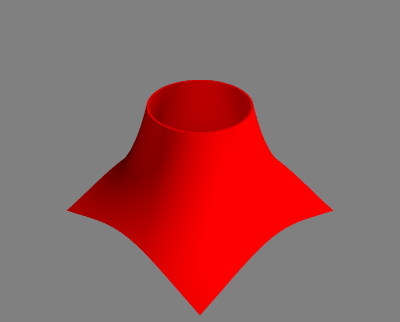
\includegraphics[width=\textwidth]{absinvz.png}
\end{subfigure}
\begin{subfigure}{.5\textwidth}
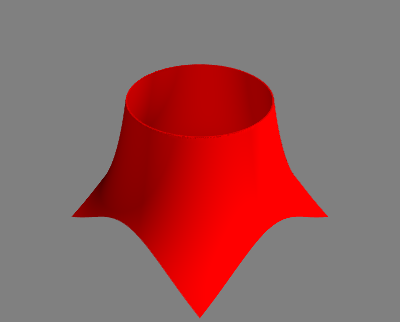
\includegraphics[width=\textwidth]{absinvz2.png}
\end{subfigure}
\caption{Surface plots of the absolute value of $\frac{1}{z}$ and $\frac{1}{z^2}$ about the origin.}
\label{fig:inv_surfaces}
\end{figure}

\begin{problem}
Write a function that takes in a function, x and y bounds, and a resolution and plots the modulus of the function as a 3d plot. Remember to take in account that it may be around a singularity.
\end{problem} 

\begin{comment}
Color plots, when used in their default form suffer from similar limitations.
On the other hand, we can do things like taking the absolute value, then scaling the values of a function logarithmically to mitigate some of the effect that the rapid growth of the plot values has on the colors in the plot.
We can also allow the color map used by the plotting library to repeat itself as the values of the function get larger and larger.
This can be done by taking the sine of the values.
Combining these things together, we obtain expressions like $\sin\left(\log\left|\text{Re}\left(Z\right)\right|\right)$.

\begin{warn}
When generating color plots like this, you will have to check for floating point values of \li{nan} and \li{inf}.
One easy way to get rid of them is to set those values to zero.
\end{warn}


\begin{problem}
Write a function that produces color plots of $\sin\left(\log\left|f\left(z\right)\right|\right)$ for a given function $f$.
Have it accept bounds for the interval where you want the plot generated.
Also have an argument that tells the function whether to use the real part, imaginary part, or the absolute value of the function.
\end{problem}
\end{comment}

\section*{Residues}
The number $a_{-1}$ in the Laurent expansion for a function $f$ at a point $z_0$ is called the Residue of $f$ at $z_0$.
The formula for the coefficients of the Laurent series provides one way to compute residues.
It is sometimes easier to evaluate a residue using limits or some other formula.
One good way to do this is to use the following formula:

Let $f(z)=\frac{p(z)}{q(z)}$ and let $p$ and $q$ be holomorphic at $z_0$. Let $p(z_0) \neq 0$ and $q(z_0)=0$.
Suppose that $z_0$ is a pole of order $1$ of $f$.
Then
\[\Res{z=z_0} f(z) = \frac{p(z_0)}{q'(z_0)}\]

A natural consequence of the Laurent series expansion of $f(z)$ and $f'(z)$ at a pole $z_0$ is that, where $d$ is the degree of the pole at $z_0$,
\[- \Res{z=z_0} \frac{f'(z)}{f(z)} = d\]
This is a useful bit of information that may be used to simplify computation of residues or of the Laurent series expansion of a function since it allows us to avoid evaluating a long series of integrals we already know will evaluate to $0$.

There is also a natural relationship between the residues of a function at its poles and its partial fraction decomposition.
Let $f = \frac{p}{q}$ where $p$ and $q$ are polynomials, $q$ has no repeated roots, and the degree of $p$ has degree less than the degree of $q$.
This means that $f$ has a partial fraction representation
\[f = \sum \frac{c_i}{z - z_i}\]
where the $c_i$ are appropriately chosen coefficients and $z_i$ are the distinct zeros of $q$.
Consider what happens when we take the residue of this sum.
Since integrals distribute over sums, so do residues, so we may say
\[\Res{z=z_i} f = \sum \Res{z=z_i} \frac{c_i}{z - z_i}\]
Since the zeros of $q$ are distinct, and the function $\frac{1}{z - z_i}$ is holomorphic wherever $z \neq z_i$, we see that
\[\Res{z=z_i} f = c_i \Res{z=z_i} \frac{1}{z-z_i} = c_i\]
This means that we can use residues to compute partial fraction decompositions, so long as the function in the denominator does not have repeated roots.

\begin{problem}
Write a Python function that, given polynomial objects $p$ and $q$, computes the partial fraction decomposition of the function $\frac{p}{q}$.
Assume that the degree of $p$ is less than the degree of $q$ and that $q$ has no repeated roots.
Return two arrays.
The first should contain the coefficients in the partial fraction decomposition.
The second should contain the corresponding zeros of $q$.

Hint: NumPy's \li{poly1d} objects have a \li{roots} attribute that allows you to quickly find the roots of a polynomial.
\end{problem}

\section*{Evaluating Indefinite Integrals Using Residues}

One convenient use of residues is the evaluation of integrals that are difficult to evaluate symbolically in other ways.
Often, when we cannot directly assign a value to one of these integrals, residues can still help us evaluate the Cauchy principal value of the integral.
Recall that, for an integral $\int_{-\infty}^{\infty} f(x)dx$, the Cauchy principal value is $\lim_{r\to \infty} \int_{-r}^{r} f(x) dx$.
This limit may exist, even though the integral itself may not.
The methods for using residues to evaluate such integrals will be discussed in greater details in the text.
Here we consider one example.

\begin{figure}
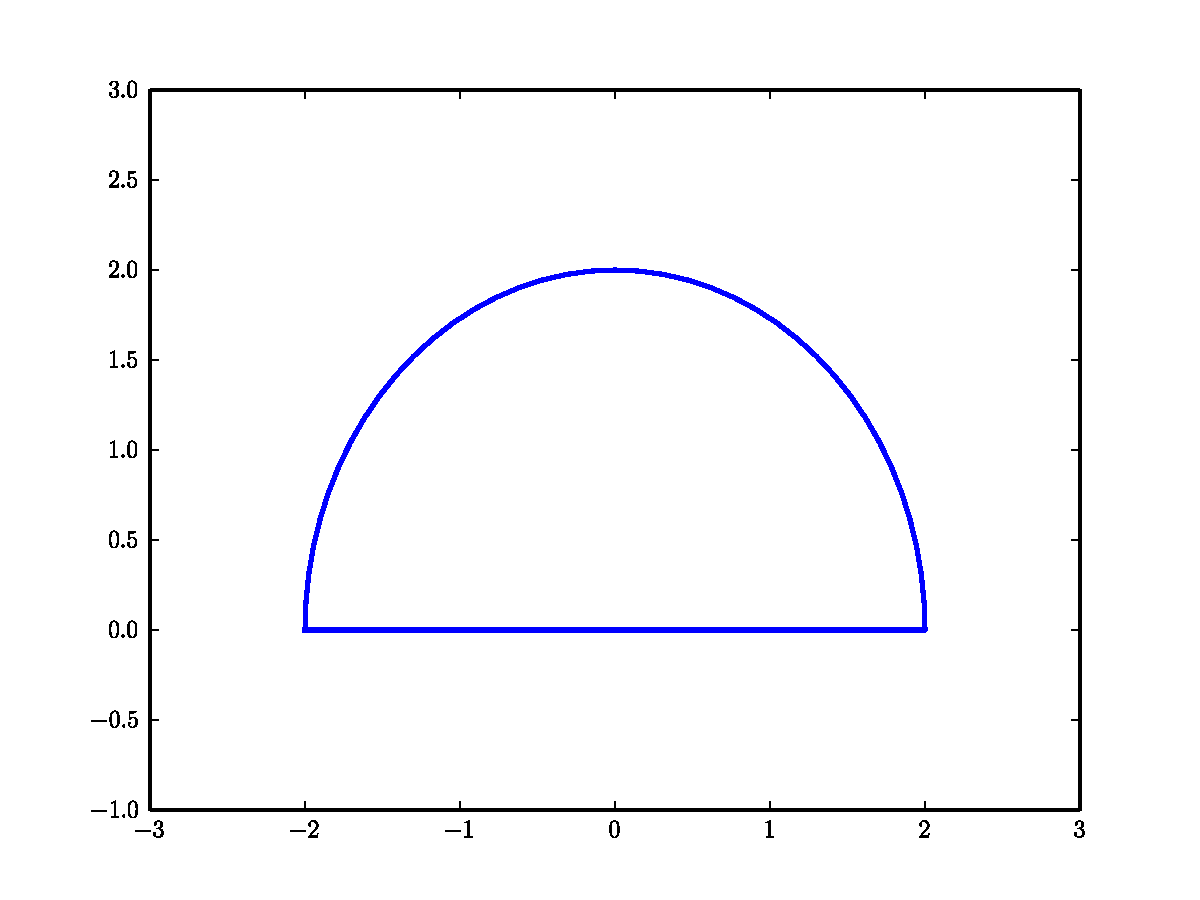
\includegraphics[width=\textwidth]{contour1.pdf}
\caption{A contour used for integration using residues.}
\label{complexint:c1}
\end{figure}

Consider the integral $\int_{-\infty}^{\infty}\frac{z^2}{z^4+1}$.
Let $f(z)=\frac{z^2}{z^4+1}$.
Notice that this function has poles at $e^{\frac{\pi i}{4}}$, $e^{\frac{3\pi i}{4}}$, $e^{\frac{5\pi i}{4}}$, and $e^{\frac{7\pi i}{4}}$.
For notation, let these be $p_1$, $p_2$, $p_3$, and $p_4$.
For some real $R>1$, consider the contour $C$ from $-R$ to $R$ and counterclockwise along the circle centered at $0$ of radius $R$ back to -$R$.

This contour (a semi circle) is shown in Figure \ref{complexint:c1} with $R = 2$.
Let $A$ be this second portion of $C$.
Note that, since $R>1$ we have
\[\int_C f(z)dz = 2\pi i (\Res{z=p_0} f(z) +\Res{z=p_1} f(z))\]
So, rewriting, we have
\[\int_{-R}^R f(z) dz = 2\pi i (\Res{z=p_0} f(z) +\Res{z=p_1} f(z)) - \int_A f(z) dz\]
so
\[\int_{-\infty}^{\infty} f(z) dz = \lim_{R\to \infty} \int_{-R}^R f(z) dz = 2\pi i (\Res{z=p_0} f(z) +\Res{z=p_1} f(z)) - \lim_{R\to \infty} \int_A f(z) dz\]
We would like to show that $\lim_{R\to\infty} \int_A f(z) dz = 0$, so note that on $A$, $\abs{z}=R$.
With some effort, it follows from the triangle inequality that $\abs{z^4+1}\geq \abs{\abs{z}^4-1} = R^4 -1$, so we have that
\[\abs{\int_A f(z) dz}\leq \int_A \abs{f(z)} dz \leq \int_A \frac{R^2}{R^4 -1}dz = \pi R \frac{R^2}{R^4-1}\]
so $\lim_{R\to\infty} \int_A f(z) dz = 0$ as desired.
This then implies that
\[\int_{-\infty}^{\infty} f(z) dz = 2\pi i (\Res{z=p_0} f(z) +\Res{z=p_1} f(z))\]
Evaluating the residues at $p_0$ and $p_1$ we have
\[\int_{-\infty}^{\infty} f(z) dz = \frac{\pi}{\sqrt{2}}\]

\begin{comment}
If a function has a singularity on the real line, we can often still evaluate the value of $\int_{-\infty}^{\infty} f(z) dz$ using a similar argument as before, but we must now indent the path along the real axis around the singularity, then, as we take the limit as our outer contour moves out toward infinity, we can let the small contour around the singularity approach the singularity.
An example of a contour like this is shown in Figure \ref{complexint:c2}.
It is centered at the origin with $R=2$ on the outer circle and $R=\frac{1}{2}$ on the inner circle.

\begin{figure}
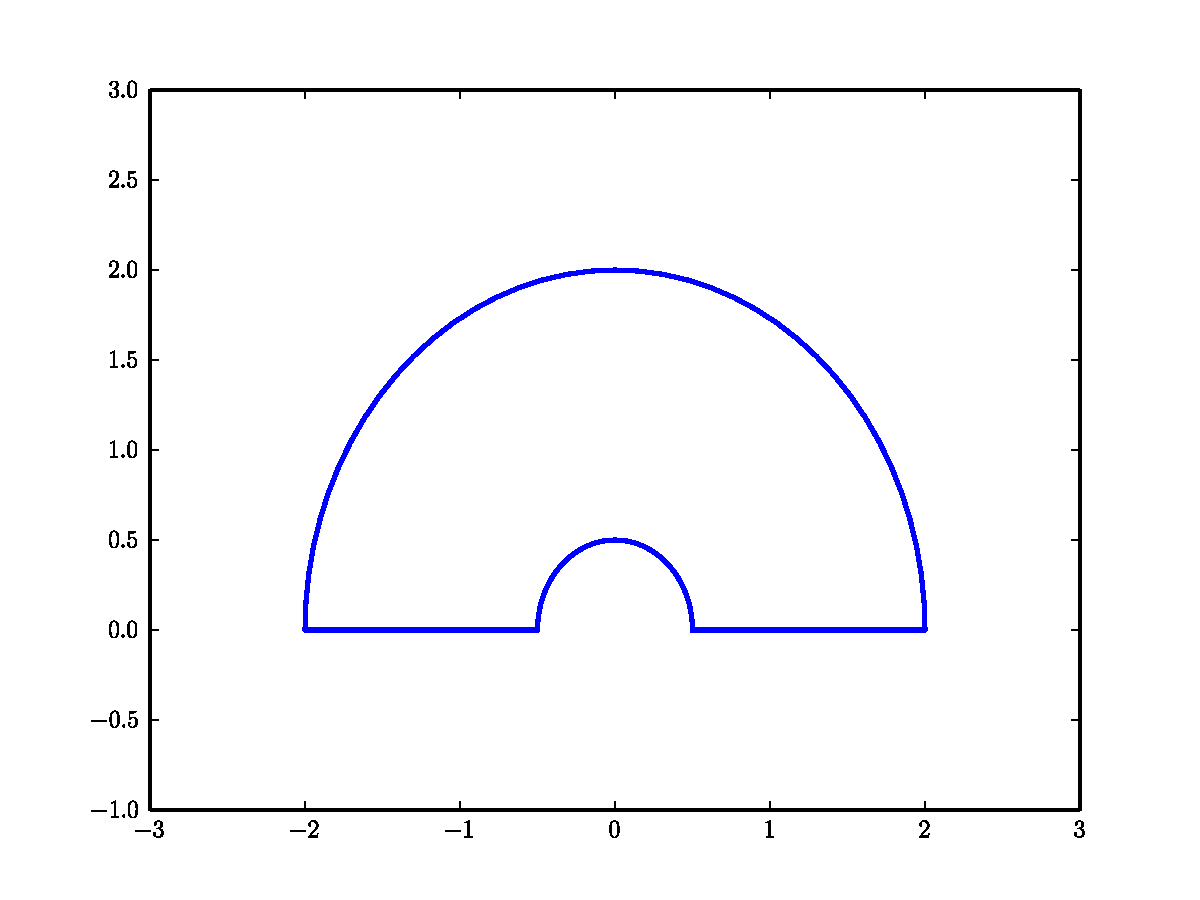
\includegraphics[width=\textwidth]{contour2.pdf}
\caption{An example of a contour that has been modified to avoid a singularity at the origin.}
\label{complexint:c2}
\end{figure}

The following is a useful theorem involving these ``indented path" methods.
\begin{theorem}
Consider a function $f$ with a pole of order $1$ at $z=x_0$ with a Laurent series representation in a punctured disk of radius $R$ about $x_0$ and residue $B_0$ at $x_0$.
Let $C_r$ be the upper half of a circle $\abs{z-x_0}=r$ where $r<R$ oriented in the clockwise direction, then
\[\lim_{r\to 0} \int_{C_r} f(z) dz = - B_0 \pi i\]
\end{theorem}
As a consequence of this, 
\end{comment}
We will not consider functions that have a singularity on the real line. So for a function $f$ on $\mathbb{C}$ with only zeros of at most order $1$ on $\mathbb{R}$, where $A$ is the sum of the residues of $f$ on the upper half plane,
\[\int_{-\infty}^{\infty} f(z) dz = 2\pi i A\]
whenever this integral exists.
When we can say that the integral of $f$ over the upper half of a circle centered at $0$ goes to $0$ as the radius of the circle increases and we can also say that the Cauchy principal value of the integral of $f$ over $\mathbb{R}$ exists, this formula will give us a proper numerical value for the Cauchy principal value of the integral of $f$ over $\mathbb{R}$.

\begin{problem}
Write a function that computes the sum $2\pi i A$ (where $A$ is defined as above) for a function $f$ of the form $\frac{p}{q}$ where $p$ and $q$ are polynomials.
\end{problem}

Integration techniques using residues can also be extended to integration around branch points, some types of integrals involving sines and cosines, inverse Laplace transforms, and many other difficult integration problems.

\begin{problem}
In the text, the zero and pole counting formula was stated and proved.
An immediate consequence of that theorem is that, for a meromorphic function $f$ and a positively oriented simple closed curve $\gamma$ that does not pass through any roots of $f$,
\[\int_\gamma \frac{f'\left(z\right)}{f\left(z\right)} dz = 2 \pi i \left(a - b\right)\]
where $a$ is the number of zeros on the interior of $\gamma$ (counting multiplicities) and $b$ is the number of poles of $f$ on the interior of $\gamma$ (also counting multiplicities).

This formula gives another possible way to count the number of zeros of a polynomial on the interior of a given contour along with looking at the color plots and manually counting them as taught in the previous lab.

Write a Python function that counts the number of zeros of a polynomial on the interior of the unit circle then plots the color plot of the function on the unit square.
\end{problem}